% ----------------------------------------------------------------- %
% AUTHOR .... Bishwa K. Giri                                    %
% CONTACT ... kirannbishwa01@gmail.com                           %
% ARTICLE ... phase-Extender/markov-chains-in-latex/          %
% UPDATED ... Apr. 29/2018                                          %
% Render this tex code on Overleaf or ShareLatex to create an image %
% ----------------------------------------------------------------- %
\documentclass{standalone}

\usepackage{tikz}
\usetikzlibrary{automata, positioning}

\begin{document}
    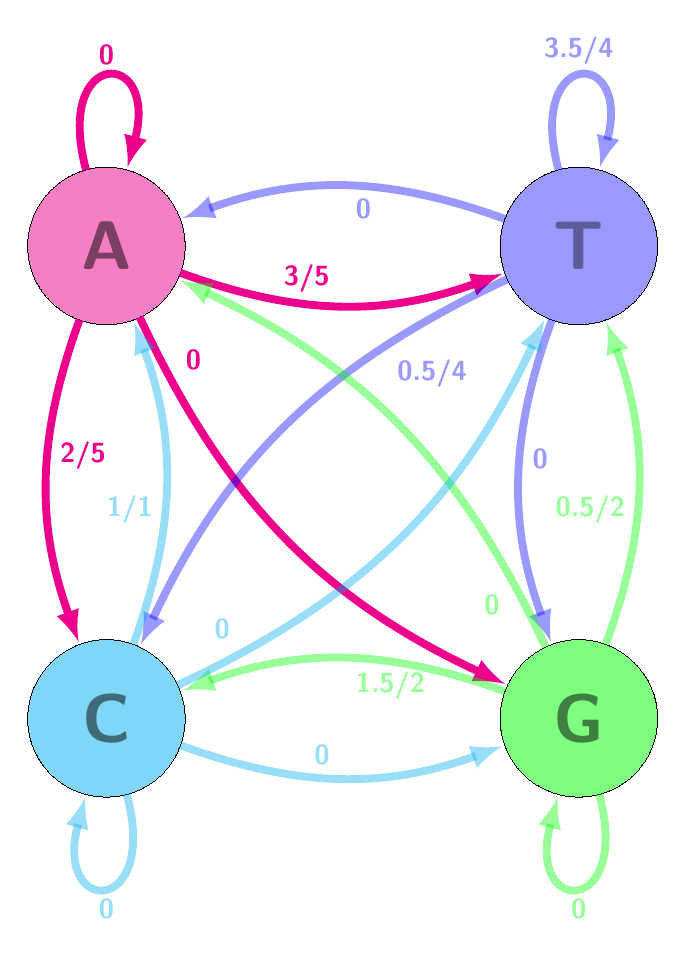
\begin{tikzpicture}[font=\sffamily]

        % Setup the style for the states
        \tikzset{node style/.style={state, 
                                    minimum width=2cm,
                                    line width=0mm,
                                    fill=white!20!white}}

        % Draw the states
        \node[node style, fill=magenta, fill opacity=0.5]
                                at (0, 0)      (A)     {\Huge \textbf{A}};
        \node[node style, fill=blue, fill opacity=0.4] 
                            at (6, 0)      (T)     {\Huge \textbf{T}};
        \node[node style, fill=green, fill opacity=0.5] 
                            at (6, -6)     (G)     {\Huge \textbf{G}};
        \node[node style, fill=cyan, fill opacity=0.5] 
                                    at (-0, -6)    (C)     {\Huge \textbf{C}};

        % Connect the states with arrows
        \draw[every loop,
              auto=right,
              line width=1mm,
              >=latex,
              draw=orange,
              fill=orange]
            (A)     edge[bend right=20, draw=magenta]  node [above left] 
            		{\color{magenta} \textbf{3/5}} (T) 
            (A)     edge[bend right=20, draw=magenta, auto=left] node [above right] 
            		{\color{magenta} \textbf{2/5}} (C)
            (A)     edge[bend right=20, draw=magenta, auto=left] node [very near start] 
            		{\color{magenta} \textbf{0}} (G)
            (A) edge[loop above, draw=magenta]  node {\color{magenta} \textbf{0}} (A)
            
            (T)     edge[bend right=20, draw=blue, opacity=0.4] node [above right] 
            		{\color{blue} \textbf{0}} (G)
            (T)     edge[bend right=20, draw=blue, opacity=0.4, auto=left] node [near start] 
            		{\color{blue} \textbf{0.5/4}} (C)
            (T)     edge[bend right=20, draw=blue, opacity=0.4, auto=left] node [below right] 
            		{\color{blue} \textbf{0}} (A)
            (T) edge[loop above, draw=blue, opacity=0.4] node {\color{blue} \textbf{3.5/4}} (T)
            
            (G)     edge[bend right=20, draw=green, opacity=0.4]    node [below right] 
            		{\color{green} \textbf{1.5/2}} (C)
            (G)     edge[bend right=20, draw=green, opacity=0.4, auto=left] node [below left] 
            		{\color{green} \textbf{0.5/2}} (T)
            (G)     edge[bend right=20, draw=green, opacity=0.4, auto=left] node [very near start] 
            		{\color{green} \textbf{0}} (A)
            (G) edge[loop below, draw=green, opacity=0.4] node {\color{green} \textbf{0}} (G)
            
            (C)     edge[bend right=20, draw=cyan, opacity=0.4, auto=left] node [below left] 
            		{\color{cyan} \textbf{1/1}} (A)
            (C)     edge[bend right=20, draw=cyan, opacity=0.4, auto=left] node [above left] 
            		{\color{cyan} \textbf{0}} (G)
            (C)     edge[bend right=20, draw=cyan, opacity=0.4, auto=left] node [very near start] 
            		{\color{cyan} \textbf{0}} (T)
            (C) edge[loop below, draw=cyan, opacity=0.4]  node {\color{cyan} \textbf{0}} (C);
    \end{tikzpicture}
\end{document}

